\scanpage{13}
\mspage{\handwritten{11}}

III Point de vue ``motivique'' en théorie du cobordisme.

Soit C la catégorie des variétés différe\unsure{\deleted{b}n|\deleted{n}b|b}tiables\inserted{\begin{tabular}[b]{@{}l@{}}\handwritten{(compactes?)}\\[-.6ex]\begin{tikzpicture}[x=1cm,y=1cm,baseline] \draw (0,-.5) .. controls (-.01,-.2) and (.02,-.12) .. (.18,-.02) .. controls (.6,.18) and (1.5,.12) .. (1.8,.17) .. controls (2.1,.19) and (2.25,.28) .. (2.23,.4); \end{tikzpicture}\end{tabular}} (pas nécessairem\unsure{e}\\
ori\unsure{e|n|a}\unsure{n|h|b}tables), \inserted{\begin{tabular}[b]{@{}l@{}}les morphismes étant les classes d'homotopie d'applications continues\\[-.6ex]\begin{tikzpicture}[x=1cm,y=1cm,line width=.4pt]\draw (.10,.40)..controls(-.18,.20)and(-.12,.02)..(.18,0)--(.67,-.02);\draw (.72,-.02)--(.77,-.02);\draw (.88,-.03)--(.94,-.03);\draw (1.08,-.03)--(1.13,-.03);\draw (1.28,-.02)--(1.46,-.02);\draw (1.68,-.02)--(1.75,-.02);\draw (1.96,-.03)--(2.02,-.03);\draw (2.18,-.04)..controls(2.43,-.07)and(2.67,-.08)..(2.78,-.19)..controls(2.83,-.29)and(2.84,-.50)..(2.81,-.53)..controls(2.66,-.23)and(2.85,-.08)..(2.95,-.05);\draw (3.02,-.04)--(3.11,-.03);\draw (3.19,-.03)--(3.29,-.03);\draw (3.39,-.03)--(3.57,-.02);\draw (3.78,-.02)--(3.88,-.03);\draw (3.97,-.03)--(4.15,-.04);\draw (4.27,-.04)--(4.31,-.04);\draw (4.40,-.04)--(4.44,-.04);\draw (4.51,-.04)--(4.94,-.02);\draw (5.06,-.02)--(5.19,-.02);\draw (5.31,-.02)--(5.50,-.02);\draw (5.62,-.02)--(5.66,-.02);\draw (5.77,-.01)--(6.05,-.01);\draw (6.23,-.01)--(6.30,-.01);\draw (6.42,-.01)--(6.47,-.01);\draw (6.59,-.01)--(6.65,-.01);\draw (6.82,-.01)--(6.89,-.01);\draw (7.04,-.01)--(7.15,-.02);\draw (7.33,-.02)--(7.44,-.02);\draw (7.55,-.02)--(7.62,-.02);\draw (7.72,-.02)--(7.80,-.02);\draw (7.98,-.03)--(8.12,-.03);\draw (8.35,-.04)--(8.47,-.04);\draw (8.60,-.04)--(8.67,-.05);\draw (8.81,-.05)--(9.05,-.06);\draw (9.17,-.06)--(9.29,-.07);\end{tikzpicture}\end{tabular}} Si B est une catégorie, on s'intéresse aux couples\\
$(F.,F^{\cdot})$ d'un foncteur covariant et d'un foncteur contravariant de C\\
dans B, satisfaisant les conditions que pour tout $X\in \mathrm{Ob}\, C$, on a $F.(X)=$\\
$F^{\cdot}(X)$, et que si on a un produit fibré ordinaire
\diagram{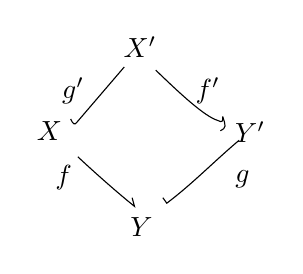
\begin{tikzpicture}[x=1cm,y=1cm,baseline] \node at (1.05,2.2) {$X'$}; \node at (-.1,1.14) {$X$}; \node at (2.45,1.12) {$Y'$}; \node at (1.07,-.08) {$Y$}; \node at (.2,1.65) {$g'$}; \node at (1.91,1.65) {$f'$}; \node at (.08,.55) {$f$}; \node at (2.35,.52) {$g$}; \draw (.85,1.95) -- (.25,1.25) .. controls (.22,1.21) and (.2,1.22) .. (.17,1.29); \draw (1.25,1.91) .. controls (1.55,1.62) and (1.87,1.32) .. (2.04,1.27) .. controls (2.09,1.24) and (2.11,1.26) .. (2.1,1.32); \draw (2.1,1.32) .. controls (2.14,1.2) and (2.15,1.18) .. (2.07,1.14); \draw (.26,.81) .. controls (.56,.53) and (.83,.3) .. (.98,.18) -- (.95,.29); \draw (2.31,1.02) .. controls (2,.76) and (1.71,.46) .. (1.39,.22) -- (1.34,.29); \end{tikzpicture}},
avec f et g transversaux, alors on a $g^{\cdot}f. = f!\,g'^{\cdot}$\inserted{\begin{tabular}[b]{@{}l@{}}(on pose $f.=F.(f)$,$f^{\cdot}=F^{\cdot}\unsure{(}$\\[-.6ex]\begin{tikzpicture}[x=1cm,y=1cm,baseline] \draw (.05,1) .. controls (-.2,.48) and (.05,.22) .. (.65,.16) -- (.95,.14) .. controls (1.1,.11) and (1.03,-.2) .. (1.08,-.62) .. controls (1.1,-.16) and (1.03,-.05) .. (1.25,.11) .. controls (2.2,.32) and (3.4,.42) .. (4.65,.24); \end{tikzpicture}\end{tabular}}. La question est\\
de trouver une B et un couple $(F.,F^{\cdot})$ qui soient ``universels'' dans \unsure{u\unsure{n}|w|u}\\
sens évident. Quillen prouve que la construction suivante donne une\\
telle solution.

Pour toute variété $X\in \mathrm{ob}\, C$ , on définit un anneau commutatif\\
B(X) (l'anneau de bordisme de X) en prenant comme éléments les class\unsure{e}\\
\deleted{de} d'éléments de C au dessus de X, pour la relation de cobordisme:\\
$f'{:}X'\rightharpoonup X$ et $f''{:}X''\rightharpoonup X$ sont équivalents, s'il existe une variété à bord\\
Z, et un $f{:}Z\to X$, tel que bord $Z = X'\handwritten{\amalg} X''$ et $f'$ et $f''$ sont induits\\
par f. La somme de B(X) est la somme disjointe (c'est une loi de grou\unsure{p}\\
\deleted{l'i\unsure{n}verse étant} où tout élément est d'ordre \deleted{1}\handwritten{2} \deleted{\unsure{ou} 2}), le produit est\\
donné par le produit fibré, en utilisant le théorème de tra\unsure{n|h|b}sversalit\unsure{e}\\
de Thom pour bouger un peu f'', de sorte à le rendre transversal à f'.
\margin{\handwritten{\uline{NB} L'anneau est de plus \uline{gradué} par la dimension relative ....}}

Si on a $f{:}\ X\rightharpoonup Y$, on définit $f. : B(X)\to B(Y)$ de façon évidente (tou\unsure{t}\\
variété sur X est sur Y), et $f^{\cdot}{:}\ B(Y)\to B(X)$ par produit fibré (uti\unsure{l}\\
sant encore le th. de transversalité). De cette façon, B(X) devient u\unsure{n|r}\\
foncteur-anneau \inserted{\begin{tabular}[b]{@{}l@{}}\handwritten{(g\unsure{ra}du\unsure{é|e})}\\[-.6ex]\begin{tikzpicture}[x=1cm,y=1cm,baseline] \draw (.12,-.9) .. controls (-.18,-.95) and (-.12,.02) .. (.2,.22) .. controls (.45,.45) and (1.1,.6) .. (1.55,.65); \draw (1.65,.65) .. controls (1.95,.73) and (2.65,.7) .. (2.85,.73) .. controls (3.15,.76) and (3.65,.97) .. (3.63,1.26); \end{tikzpicture}\end{tabular}} contravariant en X, et un foncteur groupe covariant e\unsure{n|r}

\margin{\handwritten{12}}
